\chapter{Experiment with real users}

\label{ch:experiment}

	In spite of the efforts that have been made in order to approximate human-machine dialogue through simulation, there are still complex behaviours and subtleties that could not be replicated. In this chapter the simulation results are tested with real users in a real dialogue setup as a validation. In the following, the interaction domain is presented then the experimental protocol is described. Finally, the result experiments are depicted and discussed.

\section{The Majordomo domain}

	The prototype used for the experiment (called Majordomo) has been implemented as a part of the Voicehome project at Orange Labs. This project is aimed at exploring the new opportunities that the use of the vocal modality to communicate with a smart home can bring. For that reason and in order to show that the methodology presented in this thesis is not domain dependent, this new task has been used for experiments instead of the agenda management task (event though they are somehow quite similar).
	
	Majordomo is able to program the following tasks during a specific time window:
	
	\begin{itemize}
		\item Alarm
		\item Heating
		\item Open windows
		\item Absence mode
		\item Laundry
		\item Air conditioning
		\item Swimming pool warming
		\item Swimming pool cleaning
		\item Calm mode
		\item Mow lawn
		\item Water lawn
		\item Record channel 1
		\item Record channel 2
		\item Record channel 3
		\item Hoover
		\item Run bath
	\end{itemize}
	
	However some tasks cannot be run simultaneously. For example:
	
	\begin{itemize}
		\item The lawn cannot be mowed while watered.
		\item The heating cannot be activated when the windows are open.
		\item The swimming pool cannot be warmed and cleaned at the same time.
		\item When the calm mode is activated, no hoovering nor laundry are allowed.
	\end{itemize}
	
	This is a slot-filling task where the user is supposed to provide the following information: the action type (ADD, MODIFY or DELETE), the task (see the list below), the date and the time window.

\section{Experimental protocol}

	\subsection{Implementation}
	
		The Client has been developed in the form of a website where the users are supposed to read a few instructions before starting to interact with the system. Google ASR has been chosen since it is a powerful off-the-shelf solution and does not require to develop any acoustic nor language model which is costly and which is not the focus of this work. Moreover, it is able to provide incremental partial results. However, it is still not able to provide the partial confidence scores (only the confidence score at the end of the utterance is provided).
		
		The implementation of the Service is similar to the personal agenda management case described in the previous chapters. The only difference is that home tasks are manipulated instead of events. Therefore, an open slot has been replaced with a slot where only a few alternatives are possible. Moreover, in the personal agenda management domain, no events can overlap whereas in the Majordomo domain some tasks can be run at the same time as others and others cannot. This is encoded in a compatibility matrix provided to the Service.
		
		As far as the Scheduler is concerned, similarly to the strategies developed in the simulation case, a handcrafted (version presented in Chapter \ref{ch:rl}, with no FEEDBACK\_RAW) as well as a reinforcement learning strategy have been implemented. The reinforcement learning strategy has been learned in simulation and tested directly with real users. Since Google ASR does not provide the confidence scores incrementally, this feature has been removed from the model. Finally, when transitioning from simulation to the real word, there is no need to estimate timing from the number of words so the real time has been taken into account.
		
	\subsection{Conduct of the dialogue}
	
		Once the user decides to start a dialogue, the system displays the interface depicted in Figure \ref{fig:majordomo}. A small briefing paragraph explains the task to accomplish which is also synthesised in the form of a table. Ten different scenarios were used and one of them was picked randomly at each new interaction. Similarly, the dialogue strategy is also picked randomly: the user can interact with the non-incremental strategy, with the handcrafted incremental or the reinforcement learning incremental strategy.
		
		When ready, the user clicks on the \textit{Start} button. During the interaction, the ASR is always on so the client is always listening except in the case of a system barge-in (when the system interrupts the user) when it is enabled for two seconds. This is necessary in order to make the system take the floor, otherwise, it will be immediately interrupted before the user even realises that there is an intervention.
		
		After the interaction, either the user ends the dialogue normally by saying \textit{Goodbye} or hangs up by clicking on the \textit{Hang up} button.
	
	\begin{figure*}[t]
		\centering
		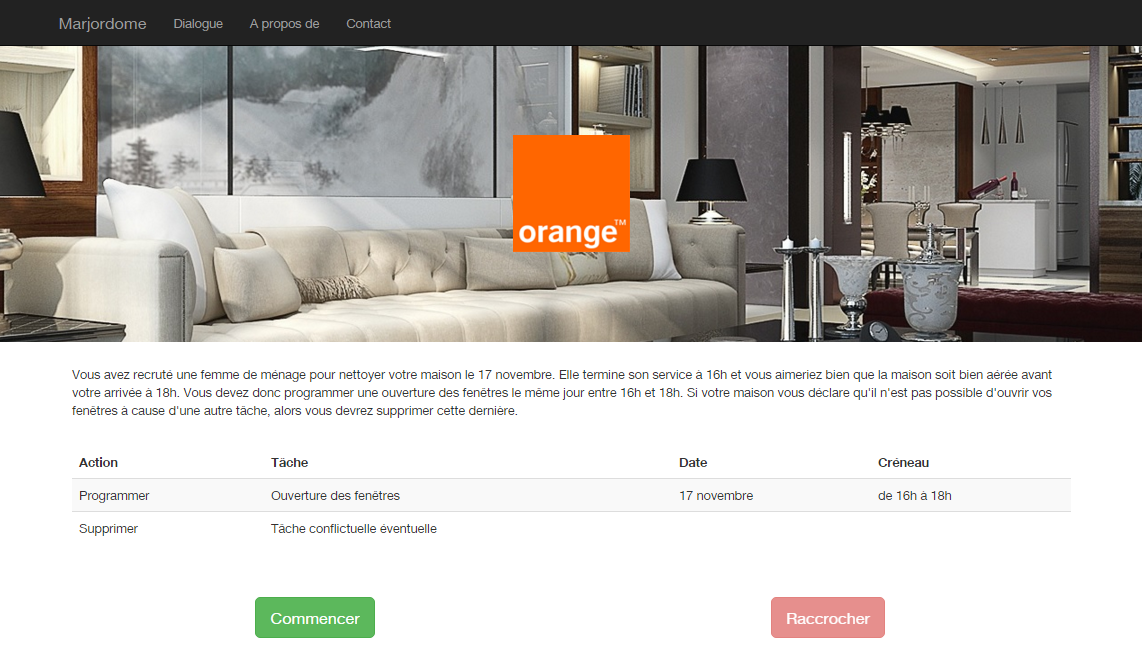
\includegraphics[scale=0.4]{figures/majordome.png}
		\caption{The Majordomo interface}
		\label{fig:majordomo}
	\end{figure*}
	
	\subsection{Key Performance Indicators}
	
		In order to evaluate the three turn-taking strategies, dialogue duration and task completion have been computed (the tasks scheduled by the Majordomo are logged at the end of the dialogue). In addition, the users filled a survey at the end of each dialogue where they provided the following subjective Key Performance Indicators (KPIs):
		
		\begin{itemize}
			\item \textbf{Reactivity:} The users are asked whether they find the system reactive or not. There are 6 possible answers going from 1 (not reactive at all, very slow) to 6 (very reactive).
			\item \textbf{Reactivity impact:} The system reactivity does not necessarily improve the dialogue quality since it can be perceived as too intrusive. The objective of this metric is to assess the impact associated with the reactivity through 6 possible values going from 1 (very negative, hurts the dialogue quality) to 6 (very positive, significant improvement of the dialogue quality).
			\item \textbf{Realism:} The users are asked whether the system acts like a human operator. There 6 possible answers going from 1 (no, not at all) to 6 (yes, clearly).
			\item \textbf{Efficiency:} The users are asked to assess the dialogue efficiency by selecting one of the 6 possible answers, going from 1 (very bad) to 6 (very good).
			\item \textbf{Global quality:} The users are asked how they globally appreciated the dialogue on a scale from 1 (Very unpleasant experience) to 6 (Very enjoyable experience).
			\item \textbf{Potential user:} Finally, the users are also asked whether they would use the Majordomo at home (if it was a real commercialised product) on a scale from 1 (clearly not) to 4 (absolutely).
		\end{itemize}


\section{Results and discussion}

	266 dialogues have been collected with the collaboration of 51 volunteer users. 81 dialogues were run using the non-incremental strategy, 90 using the handcrafted strategy and 95 using the reinforcement learning one. The experiment results are depicted in Table \ref{tab:results}.
	
	\begin{table}[th]
		\footnotesize
		\vspace{2mm}
		\centerline{
		\begin{tabular}{|c|c|c|c|c|}
			\hline
			Category & KPI & \textbf{None} & \textbf{Handcrafted} & \textbf{RL} \\
			\hline
			\multirow{2}{*}{Objective} & Duration (sec) & 110.0 & 99.5 & \textbf{97.9} \\
			& Task completion & 0.62 & 0.59 & \textbf{0.72} \\
			\hline
			\multirow{6}{*}{Subjective} & Reactivity (1-6) & 4.20 & 4.50 & \textbf{4.56} \\
			& Reactivity impact (1-6) & 4.27 & 4.20 & \textbf{4.29} \\
			& Realism (1-6) & 3.62 & \textbf{3.67} & \textbf{3.67} \\
			& Efficiency (1-6) & 4.20 & 4.18 & \textbf{4.29} \\
			& Global quality (1-6) & 4.02 & \textbf{4.17} & 4.09 \\
			& Potential use (1-4) & 2.62 & 2.66 & \textbf{2.75} \\
			\hline
		\end{tabular}
		}
		\caption{Mean values for each strategy and for each KPI}
		\label{tab:results}
	\end{table}
	
	Incremental strategies are 11\% shorter on average. At a first glance, this can be viewed as an obvious result since by construction, incremental strategies are more reactive. Nevertheless, the user can also be interrupted before she has provided all the information that she wanted which complicates the dialogue and makes it last longer like it is the case in the experiment led in \cite{Ghigi2014}. Therefore, this result shows that the Majordomo successfully interrupted the user on average. However, there is no visible change when comparing the handcrafted and the RL strategy. This trend is maintained when considering only successful dialogues (None: 107.0, Handcrafted: 95.4, RL: 93.1).
	
	As far as the task completion metric is concerned, the RL strategy offers a real advantage. It offers a gain of 10\% compared to the non-incremental baseline. The handcrafted strategy, on the other hand, degrades the latter by 3\%. When the system is reactive enough to the point that it can even interrupt the user in case of a problem, the users happen to be more engaged and more focused. This is particularly important in this task since some of the scenarios require the user to keep track of what he is doing and listen carefully to the system's responses, hence engendering an important cognitive load.
	
	From the subjective point of view, the RL strategy offers the best mean value except for the global quality metric. This is a strange result since it should be highly correlated to the task completion. An important number of users rated the dialogue for being of a good quality even though they did not finish the task. This is linked to the point made previously about the cognitive load since some users lost track of their dialogue progression with respect to the objective and then stopped the dialogue, however, they put the blame on themselves instead of the system hence giving a high global quality mark anyway.
	
	As far as statistical significance is concerned, a pairwise (none vs. handcrafted, handcrafted vs. RL and RL vs. none) Welch test has been performed (and a binomial proportions test for task completion since it is more adapted). Only the reactivity metric when the RL and the non-incremental strategies are compared showed statistically significant results since the corresponding p-value is under 0.05. The other p-values are above that threshold. As far as task completion is concerned, it is a Bernoulli random variable, hence, its variable only depends on its mean. Therefore, the only problem with the significance comes from the lack of data. For other metrics, the high variability... 
